\documentclass{article}
\usepackage{microtype}
\usepackage{graphicx}
\usepackage{subcaption}
\usepackage{booktabs}
\usepackage{hyperref}
\newcommand{\theHalgorithm}{\arabic{algorithm}}
\usepackage{icml2026}
\usepackage{amsmath}
\usepackage{amssymb}
\usepackage{mathtools}
\usepackage{amsthm}
\usepackage[capitalize,noabbrev]{cleveref}
\graphicspath{{../figures/}}
\theoremstyle{plain}
\newtheorem{proposition}{Proposition}
\theoremstyle{remark}
\newtheorem{remark}{Remark}
\newcommand{\E}{\mathbb{E}}
\newcommand{\Var}{\mathrm{Var}}
\newcommand{\dH}{d_{\mathrm H}}
\newcommand{\rrmse}{\mathrm{rRMSE}}

\icmltitlerunning{Accuracy of Regression-Based GATE Estimation Under Network Interference}

\begin{document}

\twocolumn[
  \icmltitle{How Accurate Is Regression-Based Global Effect Estimation Under Network Interference?\\
  Variance Law, Bias Floor, and Failure Modes}
  \begin{icmlauthorlist}
    \icmlauthor{Anonymous Authors}{anon}
  \end{icmlauthorlist}
  \icmlaffiliation{anon}{Anonymous Institution}
  \icmlcorrespondingauthor{Anonymous}{anonymous@example.com}
  \icmlkeywords{network interference, A/B testing, global average treatment effect, regression adjustment}
  \vskip 0.3in
]
\printAffiliationsAndNotice{}

\begin{abstract}
In A/B tests on networks, a regression-based estimator fits a model from treatment assignments (own treatment and a neighbourhood-exposure feature) to outcomes and predicts outcomes under ``everyone treated'' and ``no one treated'' to estimate the global average treatment effect (GATE). We study, by controlled simulation on synthetic graphs and two public Facebook graphs, how accurate this estimator is and what determines its error. Error splits into a sampling term and a misspecification (bias) term. For a linear-in-exposure model under Bernoulli randomisation, sampling SD follows $\hat\sigma\sqrt{(1+\dH)/(np(1-p))}$, with $\dH$ the harmonic-mean degree; this matched simulation within about 10\% when baseline outcomes are unrelated to network position, but underpredicted the SD by a factor of about 1.6--7 when baselines are community-correlated on clustered graphs or degree-correlated on hub-heavy real graphs. With a nonlinear exposure response, the linear estimator has an $n$-independent bias floor that an exact binomial formula predicts (corr.\ 0.995, 80 synthetic settings); flexible fits remove it but multiply variance. Cluster randomisation helps substantially on strongly clustered synthetic graphs but can hurt on real ones (Stanford3). Mis-specified interference structure produces predictable biases (neighbour-count channel, two-hop spillover, missing edges), and heteroskedasticity-robust CIs under-cover badly (down to 0.18) where a two-hop network-robust variant recovers 0.86--0.95 under Bernoulli designs. All conclusions are simulation-based and conditional on our outcome models.
\end{abstract}

\section{Introduction}
Online experiments on social networks and marketplaces violate the no-interference assumption: a unit's outcome depends on others' treatments. The quantity a platform usually wants is the \emph{global average treatment effect} (GATE), $\tau=\frac1n\sum_i[Y_i(\mathbf 1)-Y_i(\mathbf 0)]$, the effect of launching to everyone versus no one. The difference in means (DM) estimates something closer to the direct effect and is biased for $\tau$. A popular alternative is the \emph{regression-based} estimator \citep{chin2019,han2023}: fit $y_i\approx m(z_i,\text{exposure}_i)$ on experimental data, then evaluate $m$ at the all-treated and all-control configurations. The estimator is attractive because it is cheap and works with plain Bernoulli randomisation, but it \emph{extrapolates}: under Bernoulli($p$) assignment, almost no unit experiences an exposure near 0 or 1, yet $\tau$ is defined at exactly those points. Existing work gives properties under linear models and resampling-based inference \citep{chin2019}, and model-selection procedures \citep{han2023}, but a systematic picture of \emph{how accurate} the estimator is, \emph{what determines} its error, and \emph{where it breaks} is missing.

We provide such a picture empirically, backed by simple first-order formulas whose predictions we test against simulation. Our contributions are:
\begin{enumerate}
\item A decomposition of error into (i) a sampling term governed by an \emph{extrapolation leverage} $\Delta^2=n\,a^\top(X^\top X)^{-1}a$, which equals $(1+\dH)/(p(1-p))$ under Bernoulli designs, and (ii) an $n$-independent bias term from misspecification of the exposure response, with an exact binomial formula (\cref{sec:theory}).
\item A test of these predictions on synthetic graphs (ER, BA, Watts--Strogatz, SBM) and two real graphs (Stanford3, ego-Facebook), over $n\in[10^3,3.2\times10^4]$, degrees 4--64 and treatment probabilities 0.05--0.75, including regimes where they fail and diagnostics for why (\cref{sec:results}).
\item A comparison to DM, a Hájek/Horvitz--Thompson exposure estimator, a spline and a gradient-boosting regression, under Bernoulli, cluster and randomised-saturation designs, showing that no estimator or design is uniformly best and that the benefit of cluster designs differs sharply across graphs (large on SBM/WS, negative on Stanford3).
\item Quantified biases under three interference-model mismatches and a coverage study of heteroskedasticity-robust versus two-hop network-robust confidence intervals.
\end{enumerate}
Everything is simulation: the outcome models are ours, and we state where conclusions depend on them (\cref{sec:disc}).

\section{Related Work}
\textbf{Design-based estimation under interference.} \citet{aronow2017} and \citet{savje2021} develop inverse-probability estimators for exposure mappings and study consistency under limited interference; \citet{hudgens2008} is the classic partial-interference reference. These estimators are unbiased for a chosen exposure contrast but have large variance when the target exposure (all neighbours treated) has small probability, as we also find (\cref{sec:designs}). \textbf{Designs.} Graph cluster randomisation \citep{ugander2013,eckles2017,karrer2021} raises the probability of full exposure; randomised variants \citep{ugander2020}, rate-optimal spatial designs \citep{leung2022}, independent-set designs \citep{cai2023}, covariance-optimised designs \citep{chen2023} and staggered rollouts \citep{cortez2022} refine this. \textbf{Model-based analysis.} \citet{chin2019} introduced regression adjustment for the GATE with linear-model analysis and resampling inference; \citet{han2023} select graph- and treatment-based covariates and give block-bootstrap intervals; \citet{li2022} study estimation under random-graph asymptotics. Our work is complementary: rather than proposing a new estimator, we characterise the accuracy of the basic regression estimator across designs, graphs and interference mechanisms, stating when simple formulas predict its error and when they do not. Cross-sectional dependence-robust variance estimation \citep{conley1999} motivates our two-hop network-HAC interval.

\section{Setup, Estimators and Predictions}\label{sec:theory}
\textbf{Model.} Graph $G$ with adjacency $A$, degrees $d_i$, assignment $z\in\{0,1\}^n$, exposure $f_i=\sum_jA_{ij}z_j/d_i$. Outcomes are
\begin{equation}
Y_i(z)=b_i+\delta z_i+\beta\,h_s(f_i),
\end{equation}
where $b_i$ is a fixed baseline (community effect $+$ loading $\times$ standardised log-degree $+$ $\sigma\,\epsilon_i$), $h_s$ is a normalised sigmoid with $h_s(0)=0$, $h_s(1)=1$ and $h_0(f)=f$ (linear), so $\tau=\delta+\beta$ for every $s$. We use $\delta=\beta=1$ ($\tau=2$) throughout. Variants replace $h_s(f_i)$ by a neighbour \emph{count} channel $\sum_jA_{ij}z_j/\bar d$, or by a mixture of one- and two-hop exposure with weight $\omega$ on two hops (\cref{sec:mismatch}). The population (graph, $b$) is fixed; the only randomness is the assignment, so the target is the design-based RMSE.

\textbf{Estimators.} Each regression estimator fits OLS of $y$ on features $\phi(z_i,f_i)$ and returns $\hat\tau=\frac1n\sum_i[\hat m(1,\mathbf 1)-\hat m(0,\mathbf 0)]$, using the analyst's graph. Variants: \texttt{lin\_frac} $[1,z,f]$; \texttt{lin\_count}; \texttt{lin\_both} $[1,z,f,\text{count},\text{std.\ log-degree}]$; \texttt{quad\_frac}; \texttt{spline} (linear $+$ three hinge terms in $f$); \texttt{oracle\_h} $[1,z,h_s(f)]$ with the true $s$ (a correctly-specified reference unavailable in practice); \texttt{two\_hop} $[1,z,f,f^{(2)}]$; and \texttt{gbm}, histogram gradient boosting on $(z,f,\text{count},\text{degree})$. Baselines: DM, and a Hájek estimator over units with all neighbours treated (resp.\ all control) weighted by inverse exposure probability, computed exactly for each design \citep{aronow2017,ugander2013}; it is undefined when either group is empty.

\textbf{Designs.} Bernoulli($p{=}0.5$); cluster randomisation (Louvain clusters \citep{blondel2008}, whole clusters assigned with $p{=}0.5$); randomised saturation (cluster-level saturation $q_c\sim U(0,1)$, then Bernoulli($q_c$)).

\textbf{Metrics.} Primary: relative RMSE $\rrmse=\sqrt{\E(\hat\tau-\tau)^2}/|\tau|$, which is comparable across settings, together with its parts, bias and SD, because their different dependence on $n$ and design drives our conclusions. For inference, empirical coverage of 95\% Wald intervals. Monte-Carlo uncertainty comes from a bootstrap over replicates (a caveat: only 3--4 graph/noise populations per configuration, so population-to-population variability is not captured by these intervals).

\textbf{Error decomposition and predictions.} Let $\beta^\ast$ be the probability limit of OLS and $\tau^\ast=a^\top\beta^\ast$, $a=\phi(1,\mathbf1)-\phi(0,\mathbf0)$. Then $\hat\tau-\tau=(\tau^\ast-\tau)+a^\top(\hat\beta-\beta^\ast)$: a misspecification bias and a sampling term with variance $\approx\sigma_r^2\Delta^2/n$, where $\Delta^2=n\,a^\top(X^\top X)^{-1}a$ is a leverage-like quantity measuring how far the target configuration lies from the support of the data.

\begin{proposition}[Variance law; first-order heuristic]\label{prop:var}
Under Bernoulli($p$) assignment, linear $h$, and baseline noise independent of network position with variance $\sigma^2$, and ignoring covariance between neighbours' exposures,
\[
\Var(\hat\tau_{\mathtt{lin\_frac}})\approx\frac{\sigma^2(1+\dH)}{n\,p(1-p)},\qquad \dH=\Big(\tfrac1n\textstyle\sum_i d_i^{-1}\Big)^{-1}.
\]
\end{proposition}
\emph{Derivation sketch} (\cref{app:deriv}). $z_i$ and $f_i$ are uncorrelated with $\mathrm{Var}(z_i)=p(1-p)$, $\mathrm{Var}(f_i)=p(1-p)/d_i$; the coefficients of $z$ and $f$ then have variances $\sigma^2/(np(1-p))$ and $\sigma^2\dH/(np(1-p))$ and $\hat\tau$ sums them. The $f$-term dominates: reaching $f=1$ from the data mean $p$ is $\sqrt{d(1-p)/p}$ standard deviations of $f$. Hence error grows like $\sqrt{\dH}$, falls like $n^{-1/2}$, and a \emph{harmonic} mean (dominated by low-degree units) not the mean degree enters.

\begin{proposition}[Bias floor]\label{prop:bias}
Under Bernoulli($p$), with $f_i=\mathrm{Bin}(d_i,p)/d_i$ and nonlinear $h$, the probability limit of \texttt{lin\_frac} is
\[
\tau^\ast=\delta+\beta\,\frac{\sum_i\E[(f_i-p)h(f_i)]}{\sum_i\Var(f_i)},
\]
so the bias $\tau^\ast-\tau$ does not vanish as $n\to\infty$. As $d_i\to\infty$, $\tau^\ast\to\delta+\beta h'(p)$: the estimator reports the \emph{local} slope at the design's saturation, not the secant from 0 to 1.
\end{proposition}
This follows from the OLS normal equations (\cref{app:deriv}); we evaluate the exact binomial sum, which is more accurate than the tangent limit at finite degree.

\textbf{Hypotheses} (formulated while designing the experiments, not formally pre-registered; the two-hop and missing-edge closed forms in H4 were derived after seeing E5 output): H1 \cref{prop:var} holds when baselines are unrelated to position. H2 \cref{prop:bias} predicts the bias. H3 cluster designs lower $\Delta^2$ and the bias floor by widening the exposure range. H4 mis-specified exposure channel or graph produces bias $-\beta(1-\dH/\bar d)$ (count channel under a fraction model), $-\omega\beta$ (two-hop weight $\omega$) and $-q\beta$ ($q$ the fraction of true edges missing from the analyst's graph), derived by the same normal-equation argument. H5 heteroskedasticity-robust (HC1) CIs under-cover when units' exposures are dependent. H1 and H3 were only partly supported, as reported below.

\section{Experimental Protocol}\label{sec:protocol}
Graphs. Synthetic: Erd\H{o}s--R\'enyi (ER), Barab\'asi--Albert (BA), Watts--Strogatz (WS, rewiring 0.1), planted-partition SBM (100 blocks, $10\%$ or $30\%$ of edges between blocks); $n=10^3$--$3.2\times10^4$ (mostly 8000), mean degree 4--64. Real: Facebook100 Stanford3 \citep{traud2012,rossi2015} (largest component $n=11{,}586$, 568{,}309 edges, mean degree 98, harmonic mean 10.8) and SNAP ego-Facebook \citep{mcauley2012} ($n=4{,}039$, 88{,}234 edges, mean 43.7, harmonic 11.0, max degree 1{,}045). Louvain communities give the cluster-design clusters and the community baseline effect ($\mathrm{sd}=1$ unless stated); default noise $\sigma=1$, degree loading $0.5$.

Each configuration uses 3--4 independently generated populations (graph and baseline noise) and 100--200 assignment replicates per population; in total about $2\times10^5$ simulated experiments across six experiment families (E1 variance, E2 bias floor, E3 designs, E5 mismatch, E6 coverage, E7 diagnostic). All seeds derive from the configuration index (code and exact commands are in the supplement; the whole study took roughly 2 hours wall-clock with 36 worker processes on a shared 40-core machine). Estimators see the true graph except in the missing-edge study. Full parameter grids are in \cref{app:grids}.

\section{Results}\label{sec:results}
\begin{figure*}[t]
\centering
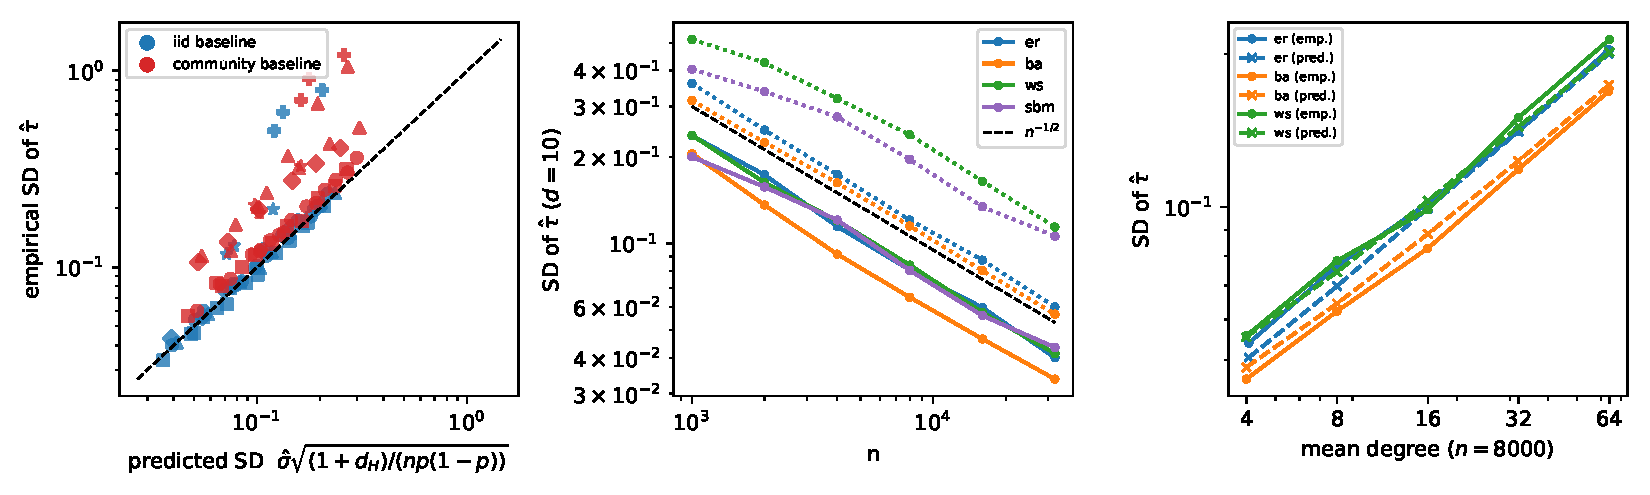
\includegraphics[width=\textwidth]{fig_varlaw.pdf}
\caption{\textbf{Sampling SD of the regression estimator (E1).} Left: empirical SD vs.\ \cref{prop:var} prediction (plug-in $\hat\sigma$); blue = iid baselines, red = community-correlated baselines; markers denote graph families. Middle: SD vs.\ $n$ ($d=10$); dotted = community baseline; dashed black slope $-1/2$. Right: SD vs.\ mean degree (iid baselines), empirical (circles) and predicted (crosses). 4 populations $\times$ 150 replicates per point.}\label{fig:varlaw}
\end{figure*}

\subsection{Sampling variance: a clean law, with identifiable failures}
\textbf{DM is badly biased, regression is not, at a price in variance.} Across all 100 E1 configurations the DM has relative bias $-0.500\pm0.001$: with $\delta=\beta$ it recovers $\delta$ only. \texttt{lin\_frac} is unbiased in these linear settings but, for iid baselines, has 1.7--8.3$\times$ the SD of DM (median about 3$\times$).

\textbf{H1 supported for position-independent baselines.} \Cref{fig:varlaw} and \cref{tab:varlaw} show that when baseline outcomes are iid, the empirical SD equals the \cref{prop:var} prediction within about 10\% (mean ratio 1.00; range 0.91--1.11 over 27 ER/BA configurations; 0.96--1.13 over 17 WS/SBM), the log-log slope in $n$ is $-0.46$ to $-0.52$, and SD grows as $\sqrt{\dH}$ with degree. On BA graphs, whose degrees are heavy-tailed, the harmonic mean matters: mean ratio 0.95 with $\dH$ vs.\ 0.82 with the mean degree; on ER/WS/SBM the two differ by at most 5 percentage points (\texttt{tables/E1\_varlaw.csv}). The same law holds on the two real graphs when baselines carry no degree dependence (ratio 0.95--1.03).

\begin{table}[t]
\caption{Empirical SD of $\hat\tau$ divided by the \cref{prop:var} prediction (mean [min, max] over configurations; E1, E7). Values near 1 mean the law works. MC error of one ratio is about 3\%.}\label{tab:varlaw}
\centering\small
\begin{tabular}{lc}
\toprule
Condition & mean [min, max] (\#configs) \\
\midrule
ER/BA, iid baseline & 1.00 [0.91, 1.11] (27) \\
ER/BA, community baseline & 1.17 [1.05, 1.30] (27) \\
WS/SBM, iid baseline & 1.04 [0.96, 1.13] (17) \\
WS/SBM, community baseline & 2.15 [1.61, 3.89] (17) \\
Real graphs, no degree loading & 0.99 [0.95, 1.03] (2) \\
Real graphs, degree loading 1.0 & 4.69 [2.30, 7.08] (2) \\
ER/BA, degree loading 1.0 & 0.92 [0.84, 1.01] (2) \\
\bottomrule
\end{tabular}

\end{table}

\textbf{...but it fails by factors of 2--7 when baselines correlate with network position.} With community-correlated baselines the ratio is 1.05--1.30 for ER/BA but 1.6--3.9 for WS/SBM, where the exposure $f_i$ is spatially smooth and nearly collinear with the community effect; the SD on WS then \emph{grows} with degree (ratio 3.9 at $d=64$) rather than following $\sqrt{d}$. On the real graphs, loading the baseline on log-degree (E7) inflates the ratio to 2.3 (Stanford3) and 7.1 (ego-Facebook, which has hubs of degree up to 1{,}045), while ER/BA with the same loading stay at 0.84--1.01. A refinement that reweights by $1/d_i$ (heteroskedastic harmonic degree, \cref{app:e7}) reduces the discrepancy on Stanford3 (2.3$\to$1.5) and BA, but leaves ego-Facebook at 5.2: our simple formulas do not explain hub-driven dependence among exposures. We did not find a closed form for this regime. Adding degree and count features (\texttt{lin\_both}) removed the inflation: its SD was 0.06--0.11 on all E7 settings, close to the no-loading value, so the variance blow-up is explainable by omitted position covariates, not by the extrapolation per se.

\subsection{Bias floor under a nonlinear exposure response}\label{sec:bias}
\begin{figure*}[t]
\centering
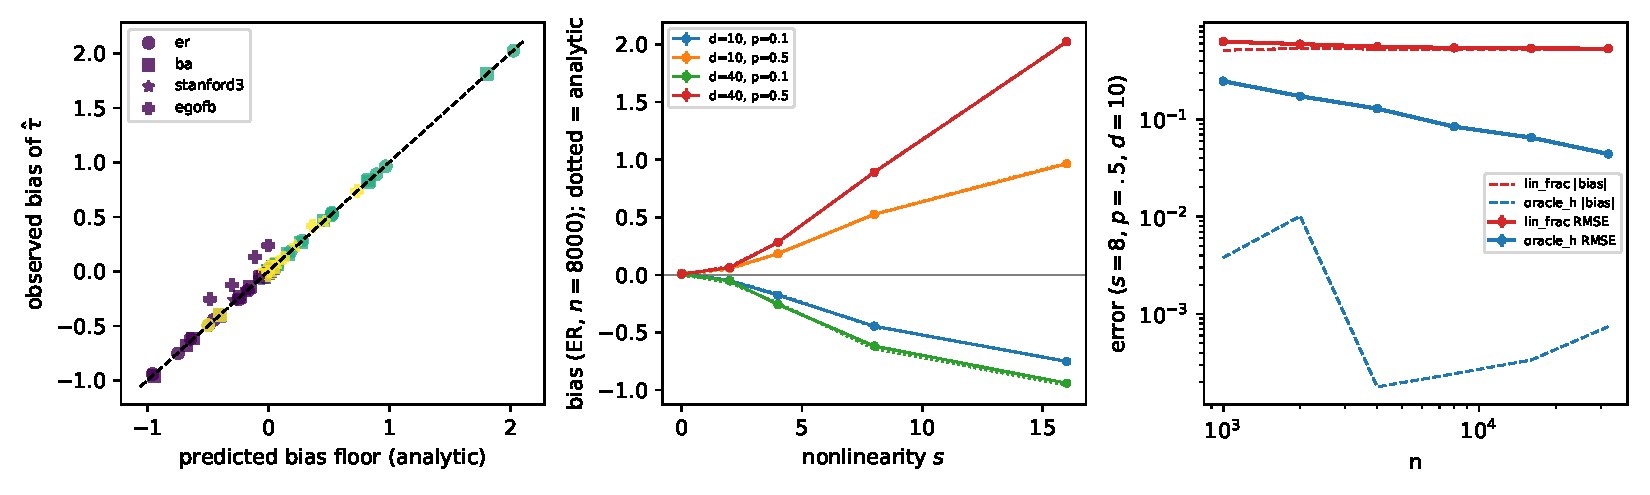
\includegraphics[width=\textwidth]{fig_bias.pdf}
\caption{\textbf{Bias floor of \texttt{lin\_frac} (E2).} Left: observed vs.\ \cref{prop:bias} bias for all E2 settings (colour = $p$). Middle: bias vs.\ nonlinearity $s$ on ER ($n=8000$); dotted = prediction. Right: error vs.\ $n$ at $s=8$, $p=0.5$, $d=10$: bias does not shrink for \texttt{lin\_frac} (red), while the correctly specified \texttt{oracle\_h} (blue) has RMSE $\propto n^{-1/2}$. Error bars: bootstrap 95\% intervals.}\label{fig:bias}
\end{figure*}
\textbf{H2 supported.} Over 80 synthetic settings (ER/BA, $d\in\{10,40\}$, $s\in\{0,2,4,8,16\}$, $p\in\{.1,.25,.5,.75\}$) the exact binomial bias of \cref{prop:bias} matches the simulated bias with mean absolute difference 0.007 and maximum 0.026 (correlation 0.995 across all 102 settings; \cref{fig:bias} left), and the prediction lies within the 95\% bootstrap interval of the observed bias in 92.5\% of the 80 synthetic cases. On Stanford3 it lies within the 95\% interval at all 8 settings; on ego-Facebook it does so for the four $p=0.5$ settings but not for the four $p=0.1$ settings (there the SD is about 1.1, and our intervals ignore between-population variation, so we do not read much into this).

\textbf{The bias is $n$-independent, signed, and depends on $p$ and $d$.} At $s=8$, $p=0.5$, $d=10$ it is $+0.53$ (26\% of $\tau$) for every $n$ from $10^3$ to $3.2\times10^4$, so RMSE plateaus at 0.53 while the correct model reaches 0.044 at $n=32000$ (\cref{fig:bias} right). Bias$^2$ exceeds variance for $n\gtrsim430$ in this setting, and in 30\% of the 80 synthetic grid settings at $n=8000$. The sign is negative at $p=0.1$ (the sigmoid is flat there, so the local slope understates the secant), small at $p=0.25,0.75$ for $d=10$ ($|\text{bias}|\le0.06$; tangent and secant happen to agree, though not at $d=40$, $s=16$: $-0.5$), and positive at $p=0.5$ where the slope is steepest (bias up to 2.0, i.e.\ 100\% of $\tau$, at $s=16$, $d=40$). Larger degree makes $f$ more concentrated and increases the bias (e.g.\ $s=8$, $p=0.5$: 0.53 at $d=10$ vs.\ 0.89 at $d=40$). The tangent limit $h'(p)$ overstates the bias at $d=40$ (tangent-limit bias 3.0 vs.\ observed 2.02 at $s=16$), so the exact binomial form is needed. Correct specification is also not enough: with $p=0.1$, $d=40$, $s=16$, \texttt{oracle\_h} has rRMSE 5.9 because the data barely identify the steep part of $h_s$ ($f\approx0.1\pm0.05$) from which it must extrapolate. A concern for practice: nothing in the observed data of a single Bernoulli experiment reveals this bias, since the fit is excellent within the observed exposure range.

\subsection{Designs and estimators}\label{sec:designs}
\begin{figure*}[t]
\centering
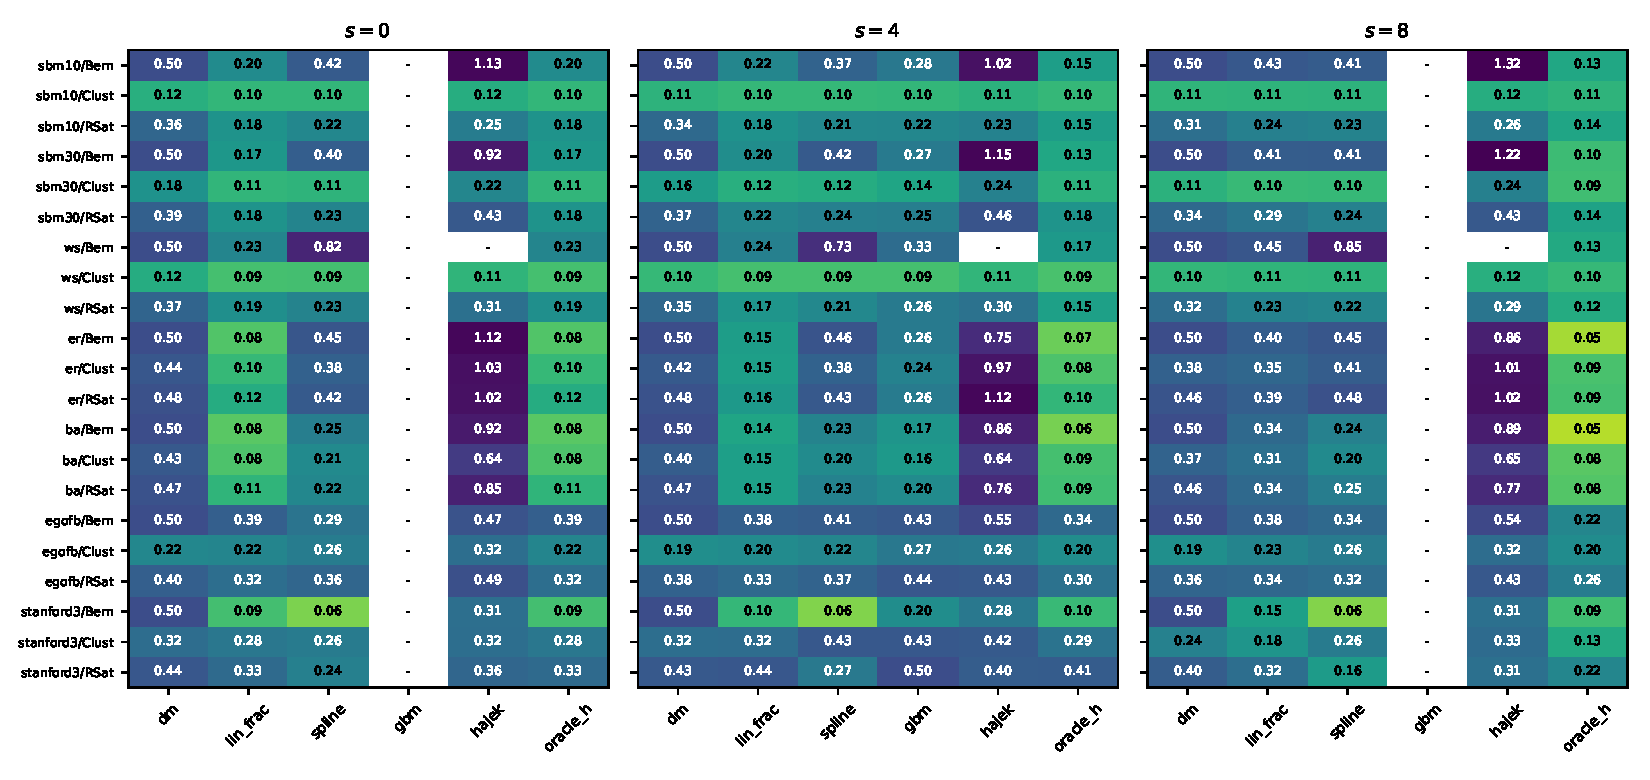
\includegraphics[width=\textwidth]{fig_designs.pdf}
\caption{\textbf{Relative RMSE by graph, design and estimator (E3).} Rows: graph/design (Bern = Bernoulli, Clust = cluster, RSat = randomised saturation); columns: estimators; panels: nonlinearity $s$. 3 populations $\times$ 100 replicates; ``--'' = undefined (GBM only run at $s=4$; Hájek always undefined in WS/Bernoulli). Colour is $\log_{10}$ rRMSE.}\label{fig:designs}
\end{figure*}
\Cref{fig:designs} summarises 63 design/graph/$s$ combinations. Findings, with the numbers behind them in \texttt{tables/E3\_metrics.csv}:
\begin{itemize}
\item \textbf{Cluster randomisation helps when clusters are real.} On SBM (10\% cross edges) and WS, where 81\% and 77\% of units have an exposure within 0.1 of 0 or 1, the extrapolation leverage drops from $\Delta^2\approx72$ (SBM) and 84 (WS) under Bernoulli to 8.1 and 6.5 under cluster randomisation and the linear estimator's bias floor disappears ($s=4$: relative bias $-0.001$ vs.\ $+0.118$ on SBM). rRMSE at $s=4$ is 0.10 vs.\ 0.22 (SBM) and 0.089 vs.\ 0.241 (WS). On ER and BA, where Louvain clusters cut many edges, $\Delta^2$ only falls from 80 to 66 (ER); cluster design brings no benefit (rRMSE 0.149 vs.\ 0.153 at $s=4$) and costs more at $s=0$ (0.101 vs.\ 0.082).
\item \textbf{On the real graphs it can hurt.} On Stanford3 cluster randomisation increases rRMSE from 0.10 (Bernoulli) to 0.32 ($s=4$; \texttt{lin\_frac}) even though $\Delta^2$ falls from 47 to 16; on ego-Facebook it helps (0.20 vs.\ 0.39, $\Delta^2$ 6.6 vs.\ 48.6) but errors stay high for both. Louvain clusters on Stanford3 retain 28\% of edges within clusters vs.\ 89\% in our SBM, and the cluster-level baseline effects ($\mathrm{sd}=1$) make the effective sample size about the number of clusters (151).
\item \textbf{Flexibility trades bias for variance, no estimator wins everywhere.} At $s=8$ on ER/Bernoulli, \texttt{lin\_frac} has rRMSE 0.40 (bias-dominated), \texttt{spline} 0.45 (variance-dominated), \texttt{oracle\_h} 0.049. At $s=0$ the spline is 2--5$\times$ worse than linear in Bernoulli designs on synthetic graphs, but better on the real graphs (Stanford3 0.06 vs.\ 0.09; ego-Facebook 0.29 vs.\ 0.39), where \texttt{lin\_frac} suffers from the degree-dependent baseline. GBM has small bias but at $s=4$ rRMSE 0.18--0.33 on synthetic Bernoulli designs vs.\ 0.06--0.17 for the oracle. On Stanford3/Bernoulli the spline wins (0.06 vs.\ 0.10--0.15 for \texttt{lin\_frac} at $s=4,8$), but on ER/BA it loses to the linear fit at $s\le4$. The ``best feasible'' estimator changes with graph, design and $s$ (\texttt{tables/E3\_best.csv}).
\item \textbf{The Hájek estimator is unusable under Bernoulli on mid-degree graphs.} With $d=20$, 97--100\% of replicates on ER/WS and 91--96\% on SBM have no fully exposed treated (or control) unit; where defined it has rRMSE $\ge0.75$. It is competitive only under cluster designs on clustered graphs (0.12 vs.\ 0.10 for \texttt{lin\_frac} on SBM).
\item \textbf{Sample size and noise.} With cluster size fixed ($\approx 80$ units; E3 sweep $n=2$k--32k, $s=4$) cluster-design RMSE falls as $n^{-1/2}$ (0.42$\to$0.11) for linear and oracle alike; Bernoulli \texttt{lin\_frac} falls from 0.74 to 0.31 but plateaus toward its bias (0.24); noise $\sigma\in[0.5,4]$ affects RMSE little for \texttt{lin\_frac} because bias or community variance dominates (\cref{app:sweeps}).
\end{itemize}

\subsection{Interference-model mismatch}\label{sec:mismatch}
\begin{figure*}[t]
\centering
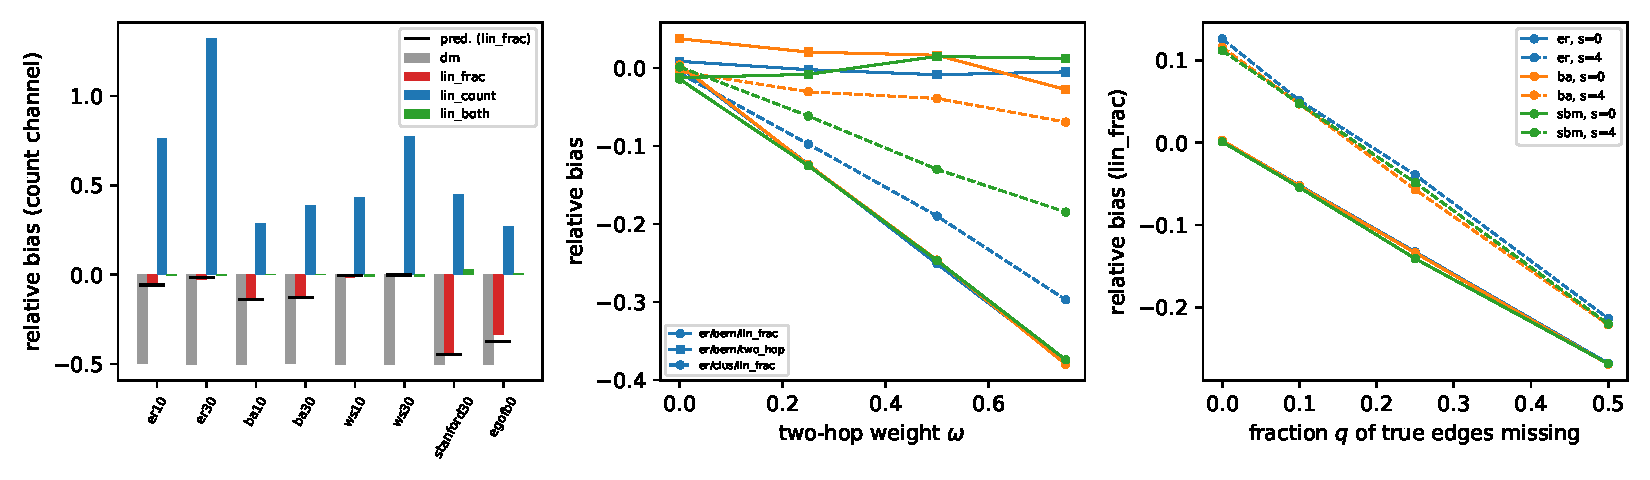
\includegraphics[width=\textwidth]{fig_mismatch.pdf}
\caption{\textbf{Mismatch biases (E5).} Left: relative bias when interference acts through the neighbour \emph{count} (bars: estimators; black ticks: $-\beta(1-\dH/\bar d)/\tau$ for \texttt{lin\_frac}). Middle: two-hop weight $\omega$ (solid: Bernoulli, dashed: cluster design); squares: the \texttt{two\_hop} estimator. Right: fraction $q$ of true edges missing from the analyst's graph (solid $s=0$, dashed $s=4$).}\label{fig:mismatch}
\end{figure*}
\Cref{fig:mismatch} and \cref{tab:mismatch} (appendix) confirm H4 quantitatively. (i) \emph{Count channel}: with true interference through the number of treated neighbours, \texttt{lin\_frac} has bias $-\beta(1-\dH/\bar d)$, e.g.\ $-0.28$ on BA ($d=10$; predicted $-0.28$), $-0.89$ on Stanford3 (predicted $-0.89$), $-0.67$ on ego-Facebook (predicted $-0.75$); it is small on near-regular graphs (ER, WS). Adding count and degree features (\texttt{lin\_both}) removes the bias ($|\text{rel.\ bias}|\le0.03$; rRMSE 0.056--0.30 vs.\ \texttt{lin\_frac} 0.09--0.55), whereas the count-only model (\texttt{lin\_count}) is wrong under the fraction model and has rRMSE up to 1.3 on ER; analysts therefore cannot pick the exposure feature from first principles. (ii) \emph{Two-hop spillover} with weight $\omega$ yields bias $-\omega\beta$ (observed $-0.25,-0.50,-0.75$ for $\omega=0.25,0.5,0.75$; Bernoulli ER); cluster designs reduce it (to $-0.06$, $-0.08$, $-0.14$ on SBM) because neighbours' and two-hop neighbours' treatments are positively correlated, so the linear fit absorbs the two-hop effect; the \texttt{two\_hop} estimator is unbiased ($|\text{rel.\ bias}|\le0.04$) but has 2--5$\times$ the RMSE for small $\omega$ (ER $\omega=0$: 0.31 vs.\ 0.09). (iii) \emph{Missing edges}: bias $\approx-q\beta$ ($-0.10$ at $q=0.1$, $-0.54$ at $q=0.5$ vs.\ predicted $-0.50$). With $s=4$ the attenuation from missing edges and the opposite-signed nonlinearity bias partially cancel (relative bias $+0.126\to-0.039$ at $q=0.25$): \texttt{lin\_frac} looks \emph{better} than the oracle there, a coincidence of errors we flag as a hazard of judging estimators by a single scenario.

\subsection{Inference}\label{sec:inference}
\begin{table}[t]
\caption{Coverage of nominal 95\% intervals for the correctly-specified regression (E6; 4 populations $\times$ 200 replicates; coverage of the true $\tau$). SE-ratio = within-population empirical SD / mean HC1 SE.}\label{tab:cov}
\centering\small
\begin{tabular}{llcccc}
\toprule
Graph & Design & $s$ & HC1 & 2-hop HAC & SE-ratio \\
\midrule
ego-FB & Bern. & 0 & 0.34 & 0.86 & 4.19 \\
ego-FB & Bern. & 4 & 0.34 & 0.86 & 4.11 \\
ego-FB & Cluster & 0 & 0.18 & 0.88 & 8.18 \\
ego-FB & Cluster & 4 & 0.20 & 0.86 & 7.31 \\
ER & Bern. & 0 & 0.88 & 0.93 & 1.22 \\
ER & Bern. & 4 & 0.88 & 0.93 & 1.22 \\
ER & Cluster & 0 & 0.59 & 0.71 & 2.34 \\
ER & Cluster & 4 & 0.55 & 0.70 & 2.56 \\
SBM & Bern. & 0 & 0.64 & 0.94 & 2.11 \\
SBM & Bern. & 4 & 0.68 & 0.95 & 2.01 \\
SBM & Cluster & 0 & 0.35 & 0.89 & 4.27 \\
SBM & Cluster & 4 & 0.31 & 0.87 & 4.86 \\
\bottomrule
\end{tabular}

\end{table}
HC1 sandwich intervals under-cover whenever exposures are dependent (\cref{tab:cov}): 0.88 on ER/Bernoulli, 0.64--0.68 on SBM/Bernoulli, and 0.18--0.34 on ego-Facebook, where the true SD is 4--8$\times$ the HC1 SE. Under cluster randomisation coverage is worse (0.31--0.59 on ER/SBM). A two-hop network-HAC estimator (sums residual cross-products over pairs within two hops) restores 0.93--0.95 for Bernoulli designs on ER/SBM and 0.86--0.88 on ego-Facebook (hubs), but is insufficient for cluster designs where dependence is cluster-wide (ER 0.70--0.71; SBM 0.87--0.89). The misspecified fits (\texttt{lin\_frac}, $s=4$) have additional bias and lower coverage (ER/Bernoulli HC1 0.72, HAC 0.79; \texttt{tables/E6\_coverage.csv}). Centring on the population-mean estimate removes bias and leaves coverage unchanged for the correct model (\texttt{covps\_*} columns), so under-coverage here is a variance-estimation failure.

\section{Discussion and Limitations}\label{sec:disc}
\textbf{What determines the accuracy.} In our simulations error is governed by three quantities: the extrapolation leverage $\Delta^2$ (set by $p$, harmonic degree and, via clusters, the exposure range), the exposure-response curvature relative to what the design reveals (bias floor), and the match between the analyst's exposure model and the true mechanism. Rules of thumb that follow, \emph{within the scope of our simulations}: expect relative error $\propto\sqrt{(1+\dH)/n}$ for linear responses and iid baselines; expect an $n$-independent bias of order $\beta|h'(p)-1|$ for sigmoid responses; compare designs with $\Delta^2$ computed from the realised $X$ rather than by default; and treat HC1 intervals as optimistic.

\textbf{Limitations.} (1) All outcome models are ours: sigmoid response of the neighbour fraction, additive baseline, $\delta=\beta=1$, and no individual-level heterogeneity in $\delta$ or $\beta$; other mechanisms (e.g.\ threshold or complier-type responses, heterogeneous spillover) may behave differently. (2) We use only 3--4 populations per configuration and the bootstrap CIs do not include population-to-population variation; ratios in \cref{tab:varlaw} carry about 3\% MC error from replicates but unknown graph-level error. (3) \cref{prop:var} is heuristic: it ignores neighbour-exposure covariance and its failure on clustered/hub graphs is characterised only descriptively; our refinement (\cref{app:e7}) is only partly successful. (4) Cluster designs use Louvain partitions with a fixed target of $\ge K$ clusters ($K=40$--100); we did not tune cluster granularity, which matters (Stanford3 vs.\ SBM). (5) Estimators with data-driven selection (e.g.\ \citealp{han2023}) were not compared; \texttt{spline}/\texttt{gbm} use fixed hyperparameters. (6) The analyst's graph is exact except in E5, and the oracle estimator uses the true $s$ so is a lower bound on achievable error. (7) The $n=64{,}000$ point of the bias-floor $n$-sweep finished in an earlier invocation, but its output was overwritten by a re-run that dropped it (it had been slow); it is not reported and the sweep stops at $n=32{,}000$. (8) The count-channel formula slightly overstates the bias on ego-Facebook ($-0.75$ vs.\ $-0.67$), probably from hub heterogeneity; we did not investigate further. (9) A GNN-type exposure feature \citep{kipf2017} was not tried.

\section*{Impact Statement}
This paper is a methodological simulation study with no human subjects or private data (public graphs only). It may help experimenters on social platforms judge when regression-based network A/B estimates can be trusted; its main risk is over-reliance on simple rules of thumb outside the simulated regimes, which we flag explicitly.

\bibliography{refs}
\bibliographystyle{icml2026}

\newpage
\appendix
\onecolumn
\section{Derivations}\label{app:deriv}
\textbf{Proposition 1.} Let $X=[\mathbf1,z,f]$, $a=(0,1,1)^\top$ and assume $y=b+\delta z+\beta f$ with $b_i$ iid mean 0 and variance $\sigma^2$ independent of $z$. Then $\hat\tau=a^\top\hat\beta$, $\Var(\hat\tau\mid z)=\sigma^2a^\top(X^\top X)^{-1}a$ and, since $\E z_i=p$, $\E f_i=p$ (no self loops), $\Var(z_i)=p(1-p)$, $\Var(f_i)=p(1-p)/d_i$ and $\mathrm{Cov}(z_i,f_i)=0$, the centred Gram matrix is $n\,\mathrm{diag}(p(1-p),\,p(1-p)\overline{d^{-1}})+O(\sqrt n)$ off the diagonal, so $a^\top(X^\top X)^{-1}a\approx\frac{1}{np(1-p)}\big(1+\overline{d^{-1}}^{-1}\big)$. Because we fix $b$ and randomise $z$ (the design-based analogue), cross-terms $\sum_{i\ne j}b_ib_j\mathrm{Cov}(f_i,f_j)$ appear that vanish in expectation over iid $b$ but not for a realised population with spatially correlated $b$; this is the term our experiments find to matter. The general leverage $\Delta^2=n\,a^\top(X^\top X)^{-1}a$ is computed numerically for any design in \texttt{tables/E3\_leverage.csv}; e.g.\ for Bernoulli designs it equals $4(1+\dH)$ for $p=0.5$ (SBM10: 72.0 vs.\ $4(1+17.05)=72.2$).

\textbf{Proposition 2.} With features $(1,z,f)$ and (population) moments $\E z=\E f=p$, $\mathrm{Cov}(z,f)=0$ and $\mathrm{Cov}(z,h(f))=0$, the OLS slope on $f$ is $\mathrm{Cov}(f,y)/\Var(f)=\beta\,\mathrm{Cov}(f,h(f))/\Var(f)$ pooled over units, and the slope on $z$ is $\delta$. Pooling over units gives the formula in \cref{prop:bias}. For $d_i\to\infty$, $f_i\to p$ and a delta-method expansion gives $\mathrm{Cov}(f,h(f))/\Var(f)\to h'(p)$.

\textbf{H4 formulas.} Count channel $g=\beta f_id_i/\bar d$ with fraction regression: $\mathrm{Cov}(f_i,f_id_i)/\Var(f_i)$ pooled gives $\beta\,\dH/\bar d$ in place of $\beta$ (since $\sum_i\mathrm{Cov}(f_i,f_id_i)=np(1-p)$ and $\sum_i\Var(f_i)=np(1-p)\overline{d^{-1}}$), hence bias $-\beta(1-\dH/\bar d)$. Two-hop mixture $(1-\omega)f_i+\omega f^{(2)}_i$ with $f^{(2)}$ uncorrelated with $f$ under Bernoulli: the slope on $f$ is $\beta(1-\omega)$, bias $-\omega\beta$. A fraction $q$ of true edges missing and $s=0$: the observed $f_i$ captures a $(1-q)$ share of the neighbourhood signal, bias $-q\beta$.

\section{Experiment grids and implementation}\label{app:grids}
All experiments: $\delta=\beta=1$ unless stated; baseline $b_i=\mathrm{comm\_sd}\cdot u_{c(i)}+\mathrm{deg\_coef}\cdot\mathrm{std}(\log d_i)+\sigma\epsilon_i$ (defaults $\mathrm{comm\_sd}=1$, $\mathrm{deg\_coef}=0.5$, $\sigma=1$), $u,\epsilon$ standard normal drawn once per population; $h_s(f)=[\mathrm{sig}(s(f-\tfrac12))-\mathrm{sig}(-\tfrac s2)]/[\mathrm{sig}(\tfrac s2)-\mathrm{sig}(-\tfrac s2)]$. OLS uses \texttt{pinv}; HC1 uses $n/(n-k)$; the network-HAC kernel sets $B_{ij}=1$ if $i,j$ are within two hops (including $i=j$) and is not guaranteed PSD (we clip negative variances at 0). 
\begin{itemize}\itemsep0pt
\item \textbf{E1} (100 configs): n-scaling (ER, BA, WS, SBM $\times$ $n\in\{1,2,4,8,16,32\}\mathrm{k}$, $d=10$) $\times$ comm\_sd $\in\{0,1\}$; degree-scaling ($n=8000$, $d\in\{4,8,16,32,64\}$; ER, BA, WS); $p\in\{.05,.1,.2,.3,.5\}$ (ER, $d=10$); real graphs $p\in\{.1,.3,.5\}$. 4 populations $\times$ 150 replicates.
\item \textbf{E2} (102 configs): ER/BA $d\in\{10,40\}$ $\times$ $s\in\{0,2,4,8,16\}$ $\times$ $p\in\{.1,.25,.5,.75\}$; real graphs $s\in\{0,4,8,16\}$, $p\in\{.1,.5\}$; $n$-sweep $s=8$, $n\in\{10^3,\dots,3.2\times10^4\}$.
\item \textbf{E3} (81 configs): 7 graphs $\times$ 3 designs $\times$ $s\in\{0,4,8\}$ (3 populations $\times$ 100 replicates; synthetic $d=20$, $n=8000$); $n$-sweep and noise sweep on SBM.
\item \textbf{E5} (56 configs): count channel (8 graphs), two-hop ($\omega\in\{0,.25,.5,.75\}$; ER/SBM/WS, $n=4000$, Bernoulli/cluster), missing edges $q\in\{0,.1,.25,.5\}$ $\times$ $s\in\{0,4\}$ (ER, BA, SBM).
\item \textbf{E6} (12 configs): ER, SBM, ego-Facebook $\times$ Bernoulli/cluster $\times$ $s\in\{0,4\}$; 4 populations $\times$ 200 replicates (ER/SBM $n=4000$, $d=10$).
\item \textbf{E7} (12 configs): degree loading $\in\{0,.5,1\}$ with comm\_sd $=0$ on Stanford3, ego-Facebook, BA, ER ($p=0.5$).
\end{itemize}

\section{Additional results}\label{app:e7}
\textbf{E7 (degree-correlated baselines).} The refined plug-in $\mathrm{Var}\approx[\E r^2+\E(r^2/d)/(\E d^{-1})^2]/(np(1-p))$ with $r_i=b_i-\bar b$ (heteroskedastic harmonic degree) gives these ratios of empirical SD to the plain law / the refined plug-in (loading $=0.5/1.0$): Stanford3 1.56/2.30 vs.\ 1.25/1.50; ego-Facebook 4.16/7.09 vs.\ 3.65/5.22; BA 0.94/0.84 vs.\ 0.98/0.94; ER 1.02/1.01 vs.\ 1.00/0.97 (\texttt{tables/E7\_degdiag.csv}). The refinement helps on BA and Stanford3 but not on ego-Facebook, where hub-induced cross-unit dependence presumably dominates (not tested further).

\begin{table}[h]
\caption{Mismatch biases in absolute units ($\tau=2$) for \texttt{lin\_frac}: predicted vs.\ observed (bootstrap 95\% CI) and rRMSE (E5).}\label{tab:mismatch}
\centering\small
\begin{tabular}{llrrr}
\toprule
Mismatch & Setting & Predicted bias & Observed bias [95\% CI] & rRMSE \\
\midrule
Count channel & ER d=10 & -0.12 & -0.11 [-0.12, -0.11] & 0.09 \\
Count channel & ER d=30 & -0.03 & -0.05 [-0.07, -0.04] & 0.11 \\
Count channel & BA d=10 & -0.28 & -0.28 [-0.29, -0.27] & 0.15 \\
Count channel & BA d=30 & -0.26 & -0.26 [-0.28, -0.25] & 0.16 \\
Count channel & WS d=10 & -0.01 & -0.03 [-0.05, -0.00] & 0.12 \\
Count channel & WS d=30 & -0.00 & -0.02 [-0.07, 0.02] & 0.27 \\
Count channel & Stanford3 & -0.89 & -0.89 [-0.92, -0.87] & 0.46 \\
Count channel & ego-Facebook & -0.75 & -0.67 [-0.73, -0.62] & 0.55 \\
\midrule
Two-hop (ER, Bern.) & $\omega=0.00$ & -0.00 & 0.00 [-0.01, 0.02] & 0.09 \\
Two-hop (ER, Bern.) & $\omega=0.25$ & -0.25 & -0.25 [-0.26, -0.23] & 0.16 \\
Two-hop (ER, Bern.) & $\omega=0.50$ & -0.50 & -0.50 [-0.52, -0.49] & 0.27 \\
Two-hop (ER, Bern.) & $\omega=0.75$ & -0.75 & -0.75 [-0.77, -0.74] & 0.39 \\
Two-hop (SBM, cluster) & $\omega=0.00$ & -- & -0.01 [-0.04, 0.01] & 0.15 \\
Two-hop (SBM, cluster) & $\omega=0.25$ & -- & -0.06 [-0.08, -0.04] & 0.15 \\
Two-hop (SBM, cluster) & $\omega=0.50$ & -- & -0.08 [-0.10, -0.05] & 0.16 \\
Two-hop (SBM, cluster) & $\omega=0.75$ & -- & -0.14 [-0.16, -0.12] & 0.16 \\
\midrule
Missing edges (ER, $s{=}0$) & $q=0.00$ & -0.00 & 0.01 [-0.01, 0.02] & 0.09 \\
Missing edges (ER, $s{=}0$) & $q=0.10$ & -0.10 & -0.10 [-0.12, -0.09] & 0.09 \\
Missing edges (ER, $s{=}0$) & $q=0.25$ & -0.25 & -0.26 [-0.28, -0.25] & 0.15 \\
Missing edges (ER, $s{=}0$) & $q=0.50$ & -0.50 & -0.54 [-0.54, -0.53] & 0.27 \\
\bottomrule
\end{tabular}

\end{table}

\section{Sample-size and noise sweeps}\label{app:sweeps}
\begin{figure}[h]
\centering
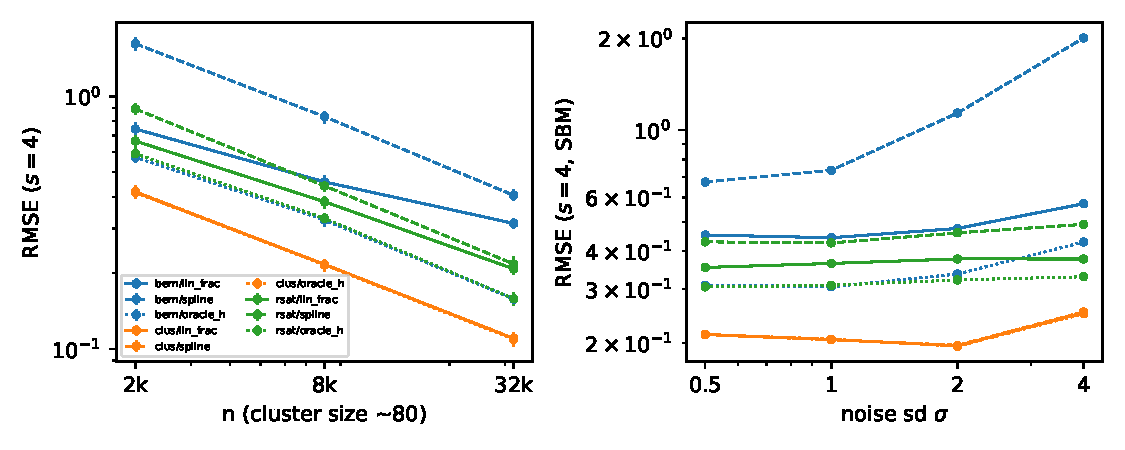
\includegraphics[width=0.6\textwidth]{fig_sweeps.pdf}
\caption{E3 sweeps on SBM ($s=4$). Left: RMSE vs.\ $n$ (cluster size $\approx80$). Right: RMSE vs.\ noise SD $\sigma$ ($d=20$, $n=8000$; the $\sigma=1$ points come from the main E3 run with 3 populations $\times$ 100 replicates, the others from separate configurations). Solid: \texttt{lin\_frac}; dashed: \texttt{spline}; dotted: \texttt{oracle\_h}; colours: Bernoulli / cluster / randomised saturation.}
\end{figure}

\section{Reproducibility and access disclosure}\label{app:repro}
Code, data-download script with checksums, seeds, commands and per-figure/table scripts are in the supplementary archive (\texttt{README.md}). Public graphs: Stanford3 from Network Repository (CC BY-SA; \texttt{socfb-Stanford3.zip}, sha256 \texttt{b1221e41...e8720d}) and SNAP ego-Facebook (\texttt{facebook\_combined.txt.gz}, sha256 \texttt{125e84db...35d7}). \textbf{Access disclosure:} while checking the existence of related work via title queries to the arXiv API, the title and author metadata of one arXiv paper on regression-based analysis of network experiments (arXiv:2309.07476) appeared in the results; it was not opened or read beyond the title line and is not cited. No other restricted material was encountered. ICML 2026 requires no separate paper checklist; we provide the Impact Statement above.

\end{document}
